\chapter{Convergence: basis order and time integration}
\label{ch:c1}
\begin{keybox}
\textbf{Key idea.} A discretization is only trustworthy if it
\emph{converges} at the rate the theory predicts --- but only if you
measure the \emph{right} error. This chapter separates the two
discretization errors so each is measured alone, controls the
\emph{algebraic} (solver) error so it cannot contaminate the plot,
verifies the reference before trusting it, and shows how the study can
lie to you.
\end{keybox}

\begin{keybox}
\textbf{Learning objectives.} By the end you can: separate spatial,
temporal, and algebraic error and measure each alone; report the
observed spatial order ($L^2\sim h^{p+1}$, $H^1\sim h^{p}$) for both
$p=1$ and $p=2$, for both fields $c$ and $\mu$; report the observed
temporal order (BDF1 $\to1$, BDF2 $\to2$) against a reference verified
by halving its $\Delta t$ and a Richardson bound; and diagnose the four
deliberate failures (wrong BC, wrong source, under-resolved feature,
under-resolved reference) that each produce a plausible but wrong
order.\\[2pt]
\textbf{Prerequisites.} The weak (FE) form and Gauss quadrature, the
method of manufactured solutions, BDF scheme order, Richardson
extrapolation; Physics Chapter~\ref{ch:p1} (the same Cahn--Hilliard
brick discretized here); Chapter~00 (environment green).\\[2pt]
\textbf{Expected cost.} Any CUDA GPU, 2-D, $<1$\,GB device memory (an
8\,GB card is ample); solver \code{splu} on the mixed $(c,\mu)$ saddle,
exact to round-off. \code{run.py} runs all four studies in
$\approx$1--2\,min on the GPU --- comparable to physics P1's quick mode,
measured $\approx75$\,s wall on an RTX~6000 Ada (mostly Warp kernel
compile + Python start-up).
\end{keybox}

This concept walks through the Cahn--Hilliard convergence gates that
ship with the solver: $p=1$ vs $p=2$ spatial order, and BDF1 vs BDF2
temporal order, each measured against a manufactured or self-convergent
reference. It connects to Physics Chapter~\ref{ch:p1} (the same brick)
and to the adaptive-stepping concept (Chapter~\ref{ch:c3}: why
variable-coefficient BDF2 matters once $\Delta t$ changes).

\section{Three errors, not one}

Every result from this simulator is wrong. The question is only
\emph{how} wrong, and whether the error shrinks --- at the rate the
theory promises --- as you refine. A time-dependent finite-element
computation carries \emph{three} errors, and a convergence study is only
meaningful when you measure one at a time:
\begin{itemize}[nosep]
  \item a \textbf{spatial} error from representing $c(\mathbf x)$ in a
        finite basis on a mesh of size $h$; for degree-$p$ elements the
        $L^2$ error scales as $h^{p+1}$ and the $H^1$ seminorm (the
        gradient error) as $h^{p}$;
  \item a \textbf{temporal} error from advancing in finite steps
        $\Delta t$; for a scheme of order $q$ it scales as
        $\Delta t^{\,q}$;
  \item an \textbf{algebraic} error from solving the nonlinear system
        only approximately (Newton stopped at some tolerance, the linear
        solve at another).
\end{itemize}
The exponents $p+1$, $p$ and $q$ are \emph{predictions}. Measuring them
is the single most important correctness check in scientific computing:
a code can run, conserve mass, and look physical while quietly
converging one order too slow because a term is missing from the weak
form. The catch is that a spatial study run with a too-large $\Delta t$
measures the \emph{time} error, and a study where Newton stopped too
early measures the \emph{solver} error --- either way you get a
wrong-but-plausible number. So we isolate each.

\section{Spatial order: a steady manufactured solution}

The trouble with checking a solver against a ``true'' answer is that
PDEs rarely have closed-form solutions. The \emph{method of manufactured
solutions} (MMS) turns the problem around: \emph{pick} a smooth field,
compute what source term would make it an exact solution, and feed that
source to the solver. Now you know the exact answer everywhere, so the
error is measurable.

The key correction over a naive MMS is to pick a \textbf{steady} (time
\emph{independent}) manufactured field. Then $c^\ast_t = 0$, the time
term contributes nothing at the discrete steady state, and the measured
error is pure spatial error --- \emph{independent of $\Delta t$}. We
manufacture composition and chemical potential independently (the
cleanest choice --- it avoids taking a Laplacian of the cubic $f'(c)$ by
hand):
%
\begin{equation}
  c^\ast = \cos(\pi x)\cos(\pi y),\qquad
  \mu^\ast = \sin(\pi x)\sin(\pi y).
\end{equation}
%
Substituting into the mixed Cahn--Hilliard system \eqref{eq:ch} leaves a
residual; we \emph{add it back} as two steady source terms so the pair
is an exact solution:
%
\begin{align}
  f_c &= -M\,\grad^2\mu^\ast = 2\pi^2 M\,\mu^\ast, \\
  f_m &= \mu^\ast - \big((c^\ast)^3 - c^\ast\big) - 2\pi^2\kappa\,c^\ast .
\end{align}
%
We impose $c^\ast,\mu^\ast$ as strong (Dirichlet) data on the boundary
(the manufactured field is not no-flux), then take a few very large
$\Delta t$ steps from the exact field: the time term $\sigma\sim1/\Delta
t$ vanishes and each Newton solve lands on the discrete \emph{steady} FE
system --- staying in the correct branch of the non-monotone cubic
$f'(c)$ (small-$\Delta t$ marching can drift to a spurious steady branch,
a real Cahn--Hilliard pitfall).

We report $L^2$ \emph{and} $H^1$ errors for \emph{both} fields $c$ and
$\mu$, plus the discrete mass error, over \ConeSpaPoneNlevels\ mesh
levels at $p=1$ and \ConeSpaPtwoNlevels\ at $p=2$ (two points is not a
study). The observed orders match theory to two figures: $L^2$ order
$p{+}1$, $H^1$ order $p$, for each field.

\begin{keybox}
\textbf{Reading a convergence order.} If the error is
$E(h)\approx C\,h^{\,k}$, then between two meshes with $h$ and $h/2$,
$\;\log_2\!\big(E(h)/E(h/2)\big) = k$. That ratio --- the
\emph{observed order} --- is what you compare against the theoretical
value. It is far more diagnostic than any single error value: the
\emph{slope} is the physics of the method; the \emph{intercept} $C$ is
just problem-dependent. We fit the slope by least squares across all
levels.
\end{keybox}

\begin{figure}[h]\centering
  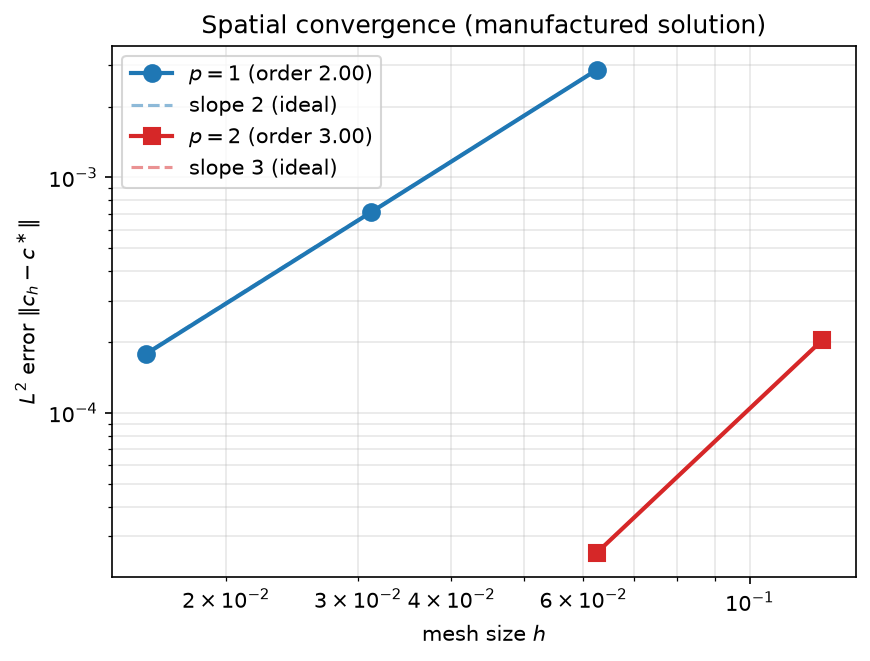
\includegraphics[width=\linewidth]{figures/c1_spatial.png}
  \caption{Spatial convergence under mesh refinement, steady MMS.
    \emph{Left:} $L^2$ error of both $c$ and $\mu$ falls along the ideal
    slope $p{+}1$ (order $\ConeSpaPoneOrder$ for $p=1$,
    $\ConeSpaPtwoOrder$ for $p=2$). \emph{Right:} the $H^1$ seminorm of
    $c$ falls one order slower, along $h^{p}$ (order
    $\ConeSpaPoneHoneOrder$ and $\ConeSpaPtwoHoneOrder$). Both fields,
    both norms, at the predicted rate.}
  \label{fig:c1spatial}
\end{figure}

\section{Algebraic error: control it, or the plot is worthless}

A convergence plot contaminated by solver error measures the solver, not
the discretization. The check is direct: hold the mesh fixed and
\emph{tighten} the Newton tolerance from $\ConeAlgTolLo$ to
$\ConeAlgTolHi$. If the measured $L^2$ error moves, the plot was
solver-limited. Here the linear solve is a direct sparse LU (\code{splu})
--- exact to round-off, so Newton is the only algebraic knob --- and the
discretization error moves by just $\ConeAlgSpread$ of itself
(Fig.~\ref{fig:c1diag}, left). The discretization error is what we claim
to measure. \emph{A study in which tightening the tolerance changes the
answer must fail this check before any order is quoted.}

\section{Temporal order: a \emph{verified} self-convergence reference}

For the time error we do not need a manufactured source. We freeze an
\emph{over-resolved} mesh, march the same smooth initial blend with a
shrinking $\Delta t$ over \ConeNdt\ levels, and compare each run against a
very fine-$\Delta t$ reference march on the identical mesh --- so the
spatial error cancels and only the time error remains. Backward Euler
(\textbf{BDF1}) is first order; the two-step \textbf{BDF2} is second
order. At constant $\Delta t$, BDF2 runs its textbook coefficients
$\tfrac{3}{2}c^{n+1} = 2c^n - \tfrac12 c^{n-1} + \Delta t\,(\cdots)$;
Chapter~\ref{ch:c3} returns to what happens when $\Delta t$ is allowed
to \emph{vary} (and why the coefficients must then change).

Self-convergence has one pitfall: if the reference is not fine enough it
is not ``truth,'' and the measured order is meaningless. So we
\emph{verify} it: halving the reference $\Delta t$ leaves the BDF2 order
unchanged ($\ConeRefOrderLo\to\ConeRefOrderHi$, a shift of
$\ConeRefStable$), and a Richardson estimate bounds the reference's own
error at $\ConeRefRich$ --- orders below the coarsest sampled error. Only
then do we trust it.

\begin{figure}[h]\centering
  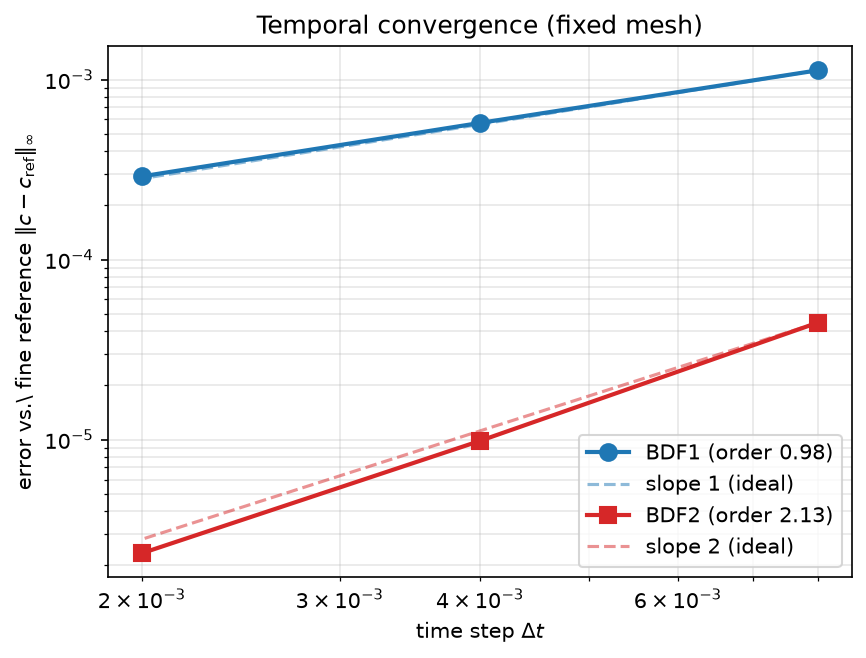
\includegraphics[width=0.82\linewidth]{figures/c1_temporal.png}
  \caption{Temporal convergence at fixed mesh. Relative $L^2$ error
    against the verified fine-$\Delta t$ reference: BDF1 tracks slope~1
    (order $\ConeBdfoneOrder$), BDF2 slope~2 (order $\ConeBdftwoOrder$).
    At the same $\Delta t$, BDF2 is over an order of magnitude more
    accurate.}
  \label{fig:c1temporal}
\end{figure}

\section{Ways to get a wrong answer}

An honest workflow includes the failure modes. Each of the following
produces a plausible-looking but \emph{wrong} order; learning to read the
signature is the skill.

\begin{figure}[h]\centering
  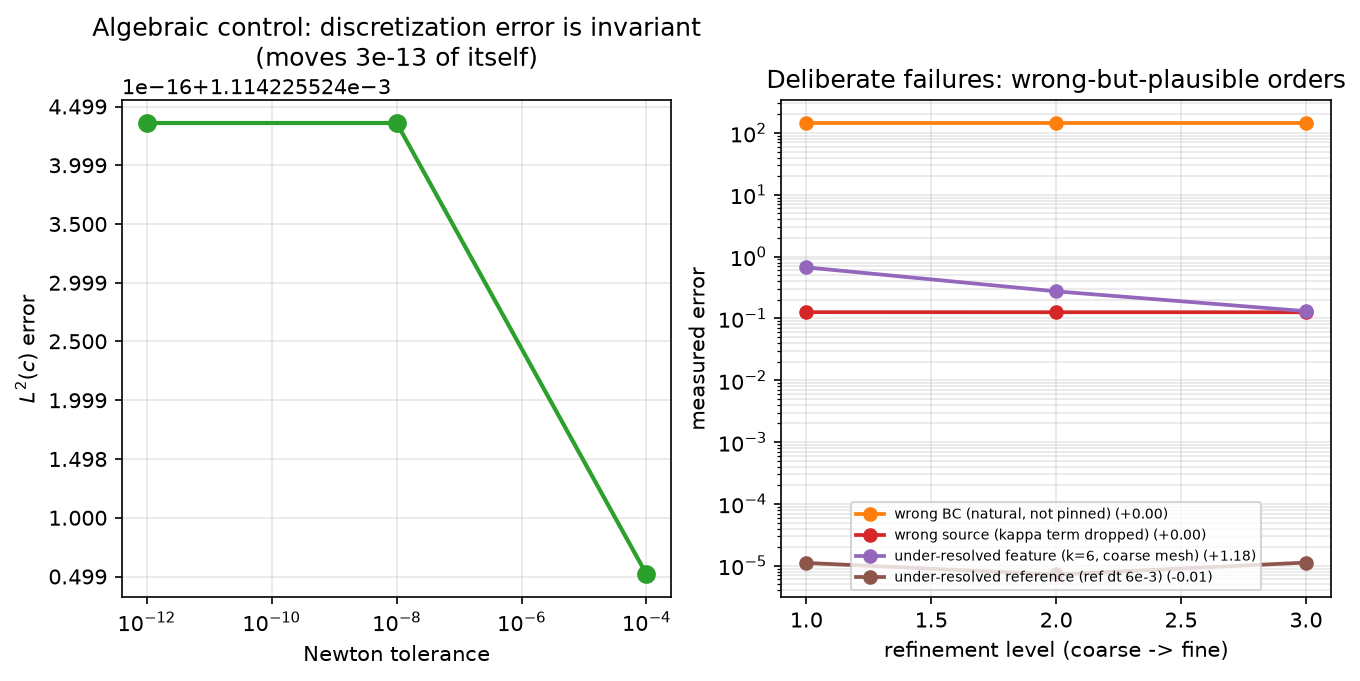
\includegraphics[width=\linewidth]{figures/c1_diagnostics.png}
  \caption{\emph{Left:} algebraic control --- the $L^2$ error is flat as
    the Newton tolerance sweeps $\ConeAlgTolLo\to\ConeAlgTolHi$
    (discretization error invariant). \emph{Right:} four deliberate
    failures, each a wrong or erratic order the student must diagnose.}
  \label{fig:c1diag}
\end{figure}

\begin{center}\small
\begin{tabular}{lcl}
\toprule
failure & measured order & signature to diagnose \\
\midrule
wrong BC (natural, not pinned) & $\ConeFailBcOrder$ & error flat and huge --- boundary dominates \\
wrong source ($\kappa$ term dropped) & $\ConeFailSrcOrder$ & converges to the \emph{wrong} steady state \\
under-resolved feature ($k{=}6$) & $\ConeFailFeatOrder$ & pre-asymptotic --- mesh cannot resolve it \\
under-resolved reference & $\ConeFailRefOrder$ & error saturates at the reference's own error \\
loose Newton (algebraic) & --- & caught by the invariance check above \\
\bottomrule
\end{tabular}
\end{center}

\noindent The last is subtle: on this smooth, well-conditioned problem
Newton converges in one or two iterations, so even a loose tolerance does
\emph{not} contaminate the order --- which is exactly why you must
\emph{verify} algebraic control rather than assume it. The lesson is not
``Newton is always fine'' but ``check, do not assume.''

\section{Run it}

\begin{runbox}
\textbf{Run it.}
\begin{lstlisting}
cd computational/01_convergence
python run.py            # spatial + algebraic + temporal + failures
\end{lstlisting}
It runs the steady-MMS spatial study ($L^2$/$H^1$ for $c$ and $\mu$), the
algebraic-control sweep, the verified temporal study for BDF1 and BDF2,
and the four deliberate failures, printing eight \code{PASS/FAIL} gate
checks. Compare with \file{EXPECTED.md} and the figures above.
\end{runbox}

\begin{keybox}
\textbf{Measured self-check} (your \file{run.py} should reproduce these
to a couple of significant figures; the observed \emph{orders} are the
load-bearing quantities). Spatial rows list $L^2(c)$ error coarse
$\to$ fine and the three fitted orders $L^2(c)$ / $H^1(c)$ / $L^2(\mu)$.
\begin{center}\small
\begin{tabular}{llcc}
\toprule
study & discretization & error (coarse $\to$ fine) & orders (expect) \\
\midrule
spatial & $p=1$ & \ConeSpaPoneErrCoarse\ $\to$ \ConeSpaPoneErrFine & $\ConeSpaPoneOrder$/$\ConeSpaPoneHoneOrder$/$\ConeSpaPoneMuOrder$ ($2/1/2$) \\
        & $p=2$ & \ConeSpaPtwoErrCoarse\ $\to$ \ConeSpaPtwoErrFine & $\ConeSpaPtwoOrder$/$\ConeSpaPtwoHoneOrder$/$\ConeSpaPtwoMuOrder$ ($3/2/3$) \\
\midrule
temporal & BDF1 & \ConeBdfoneErrCoarse\ $\to$ \ConeBdfoneErrFine & $\ConeBdfoneOrder$ ($1$) \\
         & BDF2 & \ConeBdftwoErrCoarse\ $\to$ \ConeBdftwoErrFine & $\ConeBdftwoOrder$ ($2$) \\
\bottomrule
\end{tabular}
\end{center}
Algebraic control: the error moves $\ConeAlgSpread$ of itself under a
Newton-tolerance sweep $\ConeAlgTolLo\to\ConeAlgTolHi$.
\end{keybox}

\section{Code walk-through}

The study lives in \file{convergence.py}, which drives the production
brick \file{src/diffsim/physics/cahn\_hilliard.py} --- the same brick as
Physics Chapter~\ref{ch:p1}.

\paragraph{1. Steady manufactured solution and its sources.}
\begin{lstlisting}
def c_star(x):  return cos(pi x) cos(pi y)          # time-independent
def f_c(x, t):  return 2*pi^2 * M * mu_star(x)      # residual, added back
\end{lstlisting}
\code{c\_star}, \code{mu\_star} are the exact fields; \code{f\_c},
\code{f\_m} the sources that make them exact. Because they are steady, the
measured error is pure spatial error.

\paragraph{2. Errors on the solver's quadrature.}
\begin{lstlisting}
cv, cg = st._gp_scalar(c_free)    # value + gradient at Gauss points
l2c += sum(w * (cv - c_star(xq))**2)              # L2
h1c += sum(w * ||cg - grad_c_star(xq)||**2)       # H1 seminorm
\end{lstlisting}
Integrated with the \emph{same} quadrature the solver uses --- no nodal
proxy. Both fields, both norms, plus $\int c$ for the mass error.

\paragraph{3. Algebraic control and verified reference.}
\begin{lstlisting}
algebraic_control(p=1, level=5, tols=(1e-4, 1e-8, 1e-12))  # error invariant
verify_reference(ref_dts=(2e-4, 1e-4))  # order stable + Richardson bound
\end{lstlisting}

\section{Explore on your own}

\question{Extend the $p{=}1$ spatial sweep to level~7 ($128\times128$).
Does the observed order stay at $2$? Because the study is steady the
answer is $\Delta t$-independent --- but round-off eventually floors the
error. Predict at which level the $L^2$ error stops halving-squared and
confirm it.}

\question{Change the manufactured wavenumber to $k=2$
($\cos(2\pi x)\cos(2\pi y)$). The error \emph{intercept} should jump (the
field is harder to resolve) while the \emph{order} stays $p+1$. Verify
both, and explain why the slope is invariant but the constant is not.}

\question{Reproduce the \emph{wrong-source} failure: drop the
$\kappa\,\grad^2 c$ term from \code{f\_m}. You measured order
$\ConeFailSrcOrder$ --- the scheme converges, but to the wrong steady
state. Why is a wrong-but-nonzero order more dangerous than an obvious
crash?}

\question{The under-resolved-feature failure used $k=6$ on levels
$2,3,4$ and measured order $\ConeFailFeatOrder$. Push the same field to
levels $5,6,7$ --- at what resolution does the order recover to $2$? This
is the boundary of the asymptotic range.}

\question{The $p2$ spatial study uses coarser levels ($2$--$5$) than $p1$
($3$--$6$). Count the degrees of freedom at $p{=}2$ level~4 versus
$p{=}1$ level~6 and compare the two $L^2$ errors per DOF --- which
discretization is more accurate for the same cost here?}
